%!TEX root = ../final.tex
\question Emma thinks that students can be classified either as a Berkeley
student or Stanford student by looking at each student's average number of
protests attended per semester and their average hours of sleep per night.

This scatter plot shows Emma's training set of three points for a
nearest-neighbor classifier.

\begin{figure}[h!]
  \centering
  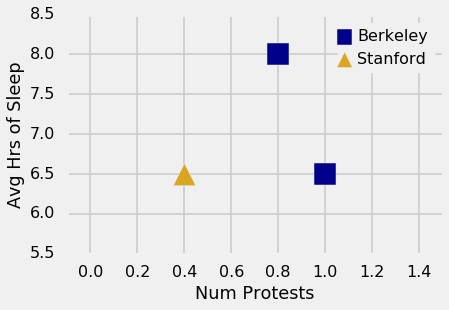
\includegraphics[scale=0.6]{class3}

  \textbf{Note that the axes are not on the same units.}
\end{figure}


\begin{parts}

\part[3] How would each unknown student be classified using a
1-nearest-neighbor classifier?

\begin{subparts}
  \subpart Student with 0.6 protests per semester and an average of 6.5 hours
  of sleep.

  \begin{oneparcheckboxes}
    \choice Berkeley
    \correctchoice Stanford
  \end{oneparcheckboxes}

  \subpart Student with 0.6 protests per semester and an average of 7.5 hours
  of sleep.

  \begin{oneparcheckboxes}
    \correctchoice Berkeley
    \choice Stanford
  \end{oneparcheckboxes}

  \subpart Student with 0 protests per semester and an average of 7.5 hours of
  sleep.

  \begin{oneparcheckboxes}
  \correctchoice Berkeley
  \choice Stanford
  \end{oneparcheckboxes}
\end{subparts}

\part[3] Draw the decision boundary for a 1-nearest neighbor classifier on the
scatterplot above.

\part[3] Suppose Emma's test set contains 100 examples all labeled Berkeley
that are distributed evenly throughout the area shown on the scatter plot
above. Which classifier will have a higher \textbf{test set} accuracy when
trained on her training set? Explain.

\begin{oneparcheckboxes}
  \choice A 1-nearest neighbor classifier
  \correctchoice A 3-nearest neighbor classifier
\end{oneparcheckboxes}

\begin{solutionorbox}[.9in]
  A 3-NN classifier will always predict Berkeley, which means it will have an
  prediction accuracy of 100\%.
\end{solutionorbox}

\part[3] Suppose Emma trains a 3-nearest neighbor classifier on her training
set. If we give the classifier a brand new point and it was classified
correctly, what is the probability that the new point was originally labeled
Stanford? Explain and show your work.

\begin{solutionorbox}[1in]
  Since a 3-NN classifier always classifies points as Berkeley, if the
  classifier was correct the point was originally labeled Berkeley with
  probability 1. This means that the probability that the point was originally
  labeled Stanford is 0.
\end{solutionorbox}

\end{parts}
